%Este trabalho está licenciado sob a Licença Creative Commons Atribuição-CompartilhaIgual 4.0 Internacional. Para ver uma cópia desta licença, visite https://creativecommons.org/licenses/by-sa/4.0/ ou envie uma carta para Creative Commons, PO Box 1866, Mountain View, CA 94042, USA.

\chapter{Conjuntos}

%Texto baseado em Topologia-Elon e \cite{munkres}.

Chamamos de \textbf{conjunto} uma coleção de objetos que satisfazem uma propriedade comum. Usaremos letras maiúsculas $A, B, \ldots$ para representar  conjuntos, e letras minúsculas $a, b, \ldots$ para representar seus elementos.

\begin{obs}
A notação $x \in A$ (lê-se ``$x$ pertence a $A$'') significa que $x$ é um elemento de $A$. A notação $x \notin A$ (lê-se ``$x$ não pertence a $A$'') significa que $x$ não é um elemento de $A$.
\end{obs}

Dados os elementos $a, e, i, o, u$ indica-se com $\{a, e, i, o, u\}$ o conjunto que é formado por estes elementos. Assim, por exemplo, $V= \{a, e, i, o, u\}$ é o conjunto das vogais do alfabeto português que pode ser denotado como um conjunto $U$.

\begin{obs}
Ao desenvolver determinado assunto de Matemática, admite-se a existência de um conjunto $U$ ao qual pertencem todos os elementos utilizados no tal assunto. Esse conjunto é chamado de \emph{conjunto universo}.
\end{obs}

No caso das vogais, podemos 

Além de relacionar elementos com conjuntos podemos relacionar dois conjuntos. Uma forma de fazer isso é através da relação de \textit{inclusão}, que é descrita da seguinte forma:

\begin{obs}
Dados dois conjuntos $A$ e $B$, diremos que $A$ está contido em $B$ (ou que $B$ contém $A$) se todo elemento de $A$ é também um elemento de $B$. Neste caso, escrevemos $A \subset B$.
\end{obs}

Note que em nosso exemplo anterior $V \subset U$, já que todas as vogais listadas também são letras do alfabeto português. Outro exemplo: como $a$ é um elemento de $V$, dizer que $a \in V$ é equivalente a afirmar que $\{a\} \subset V$.

 \begin{obs}
 Dois conjuntos $A$ e $B$ são iguais se e somente se possuem os mesmos elementos, isto é, todo elemento de $A$ é também elemento de $B$ e todo elemento de $B$ é também elemento 
 de $A$ e indica-se $A=B$. Caso $A$ não seja igual a $B$, escreve-se $A\neq B$.
 \end{obs}


Considerando três conjuntos quaisquer $A$, $B$ e $C$, a relação de inclusão entre eles possui as seguintes propriedades:

\textit{Reflexividade:} para todo conjunto $A$, tem-se que $A \subset A$.

\textit{Anti-simetria:} se $A \subset B$ e $B \subset A$, então $A= B$.

\textit{Transitividade:} se $A \subset B$ e $B \subset C$, então $A \subset C$.

\begin{obs} \emph{Notação:}
\begin{itemize}
 \item Elemento $a$ pertence ao conjunto $A$: \destaque{a \in A}.
 \item Elemento $a$ não pertence ao conjunto $A$: \destaque{a \notin A}.
  \item Conjunto $A$ é igual à $B$: \destaque{A = B}.
 \item Conjunto $A$ está contido no conjunto $B$: \destaque{A \subset B}.
 \item Conjunto $A$ contém o conjunto $B$: \destaque{A \supset B}.
 \item Conjunto $A$ é subconjunto próprio do conjunto $B$: \destaque{A \varsubsetneq B}.
 \item O conjunto que não contém nenhum elemento será chamado de conjunto vazio e denotado por \destaque{\varnothing} ou \destaque{\{ \}}.
 \item Conjunto unitário é aquele que possui um único elemento.
\end{itemize}
\end{obs}
 
 \begin{exem}
  Sejam $A= \{1, 2, 3, 4, 5 \}$ e $B=\{ 2, 3, 4\}$. Então $1 \in A$, mas $1 \notin B$. Além disso, temos que $B \subset A$ (ou ainda, que $A \supset B$), pois todos os elementos de $B$ são também elementos de $A$. Estes conjuntos serão representados através do seguinte diagrama de Venn-Euler:
 \end{exem}

 As relações entre conjuntos podem ser representadas através de diagramas de Venn-Euler (também conhecidos como diagramas de Venn), nos quais basicamente desenhamos um retângulo para representar o conjunto universo, dentro deste retângulo desenhamos um círculo para representar cada conjunto, e dentro de cada círculo escrevemos os elementos que pertencem ao conjunto correspondente.

  \begin{exem}
 Consideremos o conjunto das vogais como sendo nosso conjunto universo. Dentro dele podemos considerar os conjuntos $A= \{a,e, i\}$, e $B=\{a, o, u\}$. Estes conjuntos serão representados através do seguinte diagrama de Venn-Euler:
 \begin{center}
  \begin{venndiagram2sets}[labelOnlyA={e i},labelOnlyB={o u},labelAB={a}]
  \end{venndiagram2sets}
  \end{center}
 \end{exem}

\section{Descrição de um conjunto}
% Dados os elementos $a, e, i, o, u$ indica-se com $\{a, e, i, o, u\}$ o conjunto que é formado por estes elementos. Assim, por exemplo, $V= \{a, e, i, o, u\}$ é o conjunto das vogais do alfabeto português. Quando representamos um conjunto desta forma dizemos que estamos representando o conjunto por enumeração de seus elementos.
% Se denotarmos por $U$ o conjunto formado pelas letras do alfabeto português, e considerarmos que as vogais $a, e, i, o, u$ fazem parte deste alfabeto, podemos representar o conjunto $V$ na forma:
% \begin{equation*}
% V= \{x \in U \mid x \text{ é uma vogal}\},
% \end{equation*}
% em que $x$ representa um elemento qualquer do conjunto $U$.



% Esta segunda descrição do conjunto $V$ é uma forma usual de descrever conjuntos na matemática. Perceba que nela começamos pensando em um conjunto ``grande'' $U$ (que chamamos de conjunto universo) e em uma propriedade $P$, bem particular, que alguns elementos deste conjunto satisfazem, e assim obtemos o conjunto $V$.

% \begin{obs}
% Ao desenvolver determinado assunto de Matemática, admite-se a existência de um conjunto $U$ ao qual pertencem todos os elementos utilizados no tal assunto. Esse conjunto é chamado de \emph{conjunto universo}.
% \end{obs}


Um dos modos de se representar um conjunto é escrever os seus elementos entre chaves. Por exemplo, o conjunto formado pelos números 3,6 e 7 pode ser representado por $\{3,6,7\}$.
Este modo de representação pode ser usado para conjuntos infinitos. Por exemplo, para representar o conjunto de todos os números inteiros maiores do que 3 é o conjunto $\{4,5,6,7,8,...\}$.

Descrição por meio de uma propriedade característica dos elementos do conjunto. Pode-se representar um conjunto através de uma sentença aberta que seus elementos devem satisfazer. Para descrever um conjunto $A$ por meio de uma propriedade característica $P$ de seus elementos, devemos escrever: 
\begin{equation*}
A=\{x \mid x \mbox{ tem propriedade } P\}    
\end{equation*}
e lê-se: ``$A$ é o conjunto dos elementos $x$ tal que $x$ tem a propriedade $P$''.

Por exemplo, se denotarmos por $U$ o conjunto formado pelas letras do alfabeto português, e considerarmos que as vogais $a, e, i, o, u$ fazem parte deste alfabeto, podemos representar o conjunto $V$ na forma $V= \{x \in U \mid x \text{ é uma vogal}\}$ em que $x$ representa um elemento qualquer do conjunto $U$.


% Esta segunda descrição do conjunto $V$ é uma forma usual de descrever conjuntos na matemática. Perceba que nela começamos pensando em um conjunto ``grande'' $U$ (que chamamos de conjunto universo) e em uma propriedade $P$, bem particular, que alguns elementos deste conjunto satisfazem, e assim obtemos o conjunto $V$.

\begin{exem}
O conjunto dos estados da Região Sudeste pode ser representado por:
\begin{equation*}
    A=\{x\mid x \mbox{ é estado da Região Sudeste}\},
\end{equation*}
ou seja,
\begin{equation*}
A=\{\mbox{Rio de Janeiro}, \mbox{ São Paulo}, \mbox{ Minas
Gerais e Espírito Santo}\}.
\end{equation*}
\end{exem}

Um conjunto pode ter como elementos outros conjuntos. Por exemplo, um 
colégio é um conjunto de turmas e cada turma é um conjunto de alunos; portanto, um 
colégio é um conjunto cujos elementos são conjuntos. 
\begin{exem}
Seja $A=\{7,\{1,3\},\{3,5,8\}\}$. Este conjunto tem apenas três elementos e pode-se escrever $7 \in A$, $\{1,3\} \in A$ e $\{3,5,8\} \in A$.
\end{exem}

%\newpage
\section{Operações entre conjuntos}

Dados conjuntos arbitrários $A$ e $B$ dentro do conjunto universo $U$, definimos as seguintes operações entre estes conjuntos:

\begin{multicols}{2}
\begin{center}
 \textbf{União:}\index{Conjunto(s)!união de}
 $A \cup B=\{x \mid x \in A \text{ ou } x \in B\}.$

 \begin{venndiagram2sets}
  \fillA \fillB
 \end{venndiagram2sets}
\end{center}

\begin{center}
\textbf{Interseção:}\index{Conjunto(s)!interseção de}
 $A \cap B=\{x \mid x \in A \text{ e } x \in B\}.$

 \begin{venndiagram2sets}
  \fillACapB
 \end{venndiagram2sets}
\end{center}
\end{multicols}

\begin{multicols}{2}
 \textbf{Diferença:}\index{Conjunto(s)!diferença de}
\begin{center}
$A - B= \{x \mid x \in A \text{ e } x \notin B\}.$

 \begin{venndiagram2sets}
  \fillANotB
 \end{venndiagram2sets}
\end{center}

\phantom{Diferença}
\begin{center}
 $B - A= \{x \mid x \notin A \text{ e } x \in B\}.$

 \begin{venndiagram2sets}
  \fillBNotA
 \end{venndiagram2sets}
\end{center}
\end{multicols}


\begin{multicols}{2}
\textbf{Complementar:}\index{Conjunto(s)!complementar de}

\begin{center}
$A^{C}= \{x \in U \mid x \notin A\}$

 \begin{venndiagram2sets}
  \fillNotA
 \end{venndiagram2sets}
\end{center}

\phantom{Complementares}
 \begin{center}
 $B^{C}= \{x \in U \mid x \notin B\}$

 \begin{venndiagram2sets}
  \fillNotB
 \end{venndiagram2sets}
\end{center} 

\end{multicols}
\begin{multicols}{2}
\begin{center}
$(A\cap B)^{C}= \{x \in U \mid x \notin (A\cap B)\}$

 \begin{venndiagram2sets}
  \fillNotAorNotB
 \end{venndiagram2sets}
\end{center}

\begin{center}
$(A\cup B)^{C}= \{x \in U \mid x \notin (A\cup B)\}$
 \begin{venndiagram2sets}
  \fillNotAorB
 \end{venndiagram2sets}
\end{center}

 \end{multicols}

\begin{obs}
    Também é comum denotar o complementar de um conjunto $A$ por $\overline{A}$.
\end{obs}
 
\textbf{Produto cartesiano:}\index{Conjunto(s)!produto cartesiano de} Dados dois conjuntos $A$ e $B$, o produto cartesiano de $A$ por $B$ é o conjunto dos pares ordenados, cuja primeira entrada é um elemento de $A$ e a segunda coordenada é um elemento $B$. Este conjunto é denotado por:
\begin{equation*}
A \times B= \{(a, b) \mid a \in A \text{ e } b \in B \} \ .
\end{equation*}
 Assim por exemplo, se considerarmos $A= \{1, 2, 3\}$ e $B= \{a, b, c\}$ teremos pela definição que
\begin{equation*}
A \times B= \{(1, a), (1, b), (1, c), (2, a), (2, b), (2, c), (3, a), (3, b), (3, c)\} \ .
\end{equation*}

 O produto cartesiano de dois conjuntos pode ser representado usando eixos coordenados, como mostra o exemplo abaixo. Esta representação é particularmente útil para representar os gráficos de funções de $\R$ para $\R$.
 
 \begin{exem}
  Dados os conjuntos $A= \{1, 2, 3, 4, 5 \}$ e $B=\{ 2, 3, 4, 6\}$, podemos representá-los através do seguinte diagrama de Venn-Euler:\index{Diagrama de Venn-Euler}

  \begin{center}
  \begin{venndiagram2sets}[labelOnlyA={1 5},labelOnlyB={6},labelAB={2  3  4}]
  \end{venndiagram2sets}
  \end{center}

  Considerando os conjuntos $A$ e $B$ dados, ao aplicar as operações de conjuntos entre eles obtemos os seguintes conjuntos, e suas respectivas representações através do diagrama de Venn-Euler:

\begin{multicols}{3}
    
\begin{center}
$A \cup B=\{ 1, 2, 3, 4, 5, 6 \}$
  \begin{venndiagram2sets}[labelOnlyA={1 5},labelOnlyB={6},labelAB={2 3 4}, radius=.9cm]
  \fillA \fillB
  \end{venndiagram2sets}
\end{center}


\begin{center}
$A \cap B=\{2, 3, 4 \}$
  \begin{venndiagram2sets}[labelOnlyA={1 5},labelOnlyB={6},labelAB={2  3  4}, radius=.9cm]
  \fillACapB
  \end{venndiagram2sets}
\end{center}


\begin{center}
$A - B= \{1, 5 \}$
  \begin{venndiagram2sets}[labelOnlyA={1 5},labelOnlyB={6},labelAB={2  3  4}, radius=.9cm]
  \fillANotB
  \end{venndiagram2sets}
\end{center}

\end{multicols}

  \begin{eqnarray*}
  A \times B = \{
  (1, 2), (1, 3), (1, 4), (1, 6), (2, 2), (2, 3), (2, 4), (2, 6), (3, 2), (3, 3),
  \\
  (3, 4), (3, 6), (4, 2), (4, 3), (4, 4), (4, 6), (5, 2), (5, 3), (5, 4), (5, 6) \}
  \end{eqnarray*}

  \begin{figure}[H]
 \centering
    %\fbox{\includegraphics[width=7cm]{./cap_conjuntos/figs/ProdCartConj}}
    \caption{Produto cartesiano dos conjuntos $A$ e $B$.}
  \end{figure}

 \end{exem}

\section{Cardinalidade de conjuntos}

 A \textbf{cardinalidade}\index{Conjunto(s)!cardinalidade de}\index{Conjunto(s)!número de elementos de} de um conjunto $A$ qualquer é o número de elementos deste conjunto, e pode ser denotada por $n(A)$, $|A|$ ou $\# A$.

 Note que: $n(\varnothing)= \# \varnothing= 0$.

 É importante observar que, dados quaisquer conjuntos $A$ e $B$:
 
 A cardinalidade da união de $A$ e $B$ é dada por:
\begin{equation*}
n(A \cup B)= n A + n B - n(A \cap B) .
\end{equation*}

 Esta fórmula irá nos ajudar a resolver muitos problemas de teoria de conjuntos.

 \section{Conjunto das partes}

 Dado um conjunto $A$, o conjunto das partes de $A$, denotado por $\mathcal{P}(A)$, é o conjunto de todos os subconjuntos de $A$, ou seja,
\begin{equation*}
\mathcal{P}(A)= \{X \mid X \text{ é um subconjunto de } A\} \ .
\end{equation*}

 Dado um conjunto $A$ qualquer, precisamos ficar atentos a duas coisas:
 \begin{itemize}
 \item O conjunto $\varnothing$ sempre está no conjunto das partes de $A$, pois $\varnothing \subset A$;
 \item O conjunto $A$ sempre está no conjunto das partes de $A$, pois $A \subset A$.
 \end{itemize}
 Portanto, $\varnothing \in \mathcal{P}(A)$ e $A \in \mathcal{P}(A)$.

 \begin{exem}\label{ex:partes-abc}
 Se considerarmos o conjunto $A= \{a, b, c\}$, teremos pela definição acima que o conjuntos das partes de $A$ é:
\begin{equation*}
\mathcal{P}(A)= \{ \varnothing, \{a\}, \{b\}, \{c\}, \{a, b\}, \{a, c\}, \{b, c\}, \{a, b, c\} \} \ .
\end{equation*}
 \end{exem}

 E como sabemos se este conjunto acima contém, de fato, todos os subconjuntos do conjunto $A$? Podemos verificar isso utilizando a seguinte propriedade do conjunto das partes:

\begin{prop}
  Se o conjunto $A$ tem $n$ elementos, então $\mathcal{P}(A)$ tem $2^n$ elementos. Ou seja:
\begin{equation*}
\# A= n \ \ \Rightarrow \ \ \# \mathcal{P}(A)= 2^n \ .
\end{equation*}
\end{prop}
 \begin{proof}
 Nesta demonstração utilizaremos o princípio fundamental da contagem\index{Princípio fundamental da contagem} para contar quantos subconjuntos um conjunto $A$ com $n$ elementos tem.

 Para começar, considere um subconjunto $B$ qualquer de $A$. Observe que para cada um dos $n$ elementos de $A$, só existem duas possibilidades:
 \begin{itemize}
 \item Ou o elemento pertence ao subconjunto $B$;
 \item Ou o elemento não pertence ao subconjunto $B$.
 \end{itemize}

 Logo, pelo princípio fundamental da contagem, nós podemos montar o conjunto $B$ de
\begin{equation*}
\underbrace{2 \cdot 2 \cdot 2 \cdots 2}_{n \mbox{ vezes}}= 2^n
\end{equation*}
 maneiras diferentes.

 Portanto, há $2^n$ subconjuntos de $A$ em $\mathcal{P}(A)$.
 \end{proof}

 No Exemplo \ref{ex:partes-abc}, temos que $\# A= 3$. Logo, aplicando esta propriedade, obtemos que $\# \mathcal{P}(A)= 2^3= 8$, que é exatamente a quantidade de elementos que listamos no conjunto $\mathcal{P}(A)$. Podemos com isso concluir que estes são todos os subconjuntos do conjunto $A$ que existem, isto é, o conjunto $\mathcal{P}(A)$ está completo.


 \section{Propriedades das operações entre conjuntos}
 \index{Conjunto(s)!propriedades das operações entre}
 \index{Propriedades!das operações entre conjuntos}

Sejam $A$, $B$ e $C$ conjunto arbitrários.

\subsection{Propriedades da União}

\begin{itemize}
    \item Idempotente: $A\cup A= A$;
    \item Elemento neutro: $A\cup \varnothing = A$;
    \item Comutativa: $A\cup B = B\cup A$;
    \item Associativa: $(A\cup B)\cup C= A\cup (B\cup C)$;
    \item $A\cup U=U$.
\end{itemize}

\subsection{Propriedades da Interseção}

\begin{itemize}
    \item Idempotente: $A\cap A= A$;
    \item Elemento neutro: $A\cap U = A$;
    \item Comutativa: $A\cap B = B\cap A$;
    \item Associativa: $(A\cap B)\cap C= A\cap (B\cap C)$;
    \item $A\cap \varnothing=\varnothing$.
\end{itemize}

\begin{obs}
    Se $A\cap B=\varnothing$ então dizemos que $A$ e $B$ são disjuntos.
\end{obs}

\subsection{Propriedades da Diferença}

\begin{itemize}
    \item $A-A= \varnothing$;
    \item $A-\varnothing = A$;
    \item Em geral, $A- B \neq B - A$;
    \item $U-A = A^C$.
\end{itemize}

\subsection{Propriedades do complementar de um conjunto}

\begin{itemize}
    \item $(A^C)^C= A$;
    \item $\varnothing^C = U$;
    \item $U^C=\varnothing$;
    \item $(A\cup B)^C= A^C\cap B^C$;
    \item $(A\cap B)^C= A^C\cup B^C$;
\end{itemize}

\subsection{Outras propriedades}
\begin{itemize}
 \item $\varnothing \subset A$
 \item $A \cup \varnothing= A$ e $A \cap \varnothing= \varnothing$
 \item $A \cap (B \cup C) = (A \cap B) \cup (A \cap C)$
 \item $A \cup (B \cap C) = (A \cup C) \cap (A \cup C)$
 \item $A - (B \cup C) = (A - B) \cap (A - C)$ \emph{(lei de De Morgan)}
 \item $A - (B \cap C) = (A - B) \cup (A - C)$ \emph{(lei de De Morgan)}
 % \item $\bigcap_{\alpha \in J}(A_{\alpha} \cap B) = (\bigcap_{\alpha \in J} A_{\alpha}) \cap B$

%\begin{equation*}
%(A_1 \cap B) \cap \cdots \cap (A_n \cap B) = (A_1 \cap \cdots \cap A_n) \cap B
%\end{equation*}
 % \item $\bigcup_{\alpha \in J}(A_{\alpha} \cap B) = (\bigcup_{\alpha \in J} A_{\alpha}) \cap B$

%\begin{equation*}
%(A_1 \cap B) \cup \cdots \cup (A_n \cap B) = (A_1 \cup \cdots \cup A_n) \cap B
%\end{equation*}

 % \item $(U \times V) \cap (A \times B) = (U \cap A) \times (V \cap B)$

 % \item $X - \bigcap_{\alpha \in J} A_{\alpha} = \bigcup_{\alpha \in J}(X - A_{\alpha})$

 % \item $X - \bigcup_{i= 1}^{n} A_i = \bigcap_{i = 1}^{n}(X - A_i)$
\end{itemize}

\section{Problemas envolvendo conjuntos}

\begin{exem}
    Uma escola com 400 alunos propôs a oferta de dois cursos opcionais: Teatro e Robótica. Do total de alunos, 250 matricularam-se em Teatro, 200 matricularam-se em Robótica e 150 matricularam-se em ambos os cursos.
    Quantos alunos não se matricularam nesses cursos?

    Para resolver este tipo de problemas, podemos considerar o conjunto universo $U$ de alunos, os conjuntos $T$ e $R$ dos alunos que se matricularam em teatro e robótica, respectivamente. Pelos dados, extraímos as sequintes informações: $n(U)=400$, $n(T)=250$, $n(R)=200$ e $n(T\cap R)=150$. Para simplificar o estudo, podemos preencher o diagrama de Venn com o total de alunos da seguinte maneira:
    \begin{center}
    \begin{venndiagram2sets}[labelA=$T$, labelB=$R$,labelOnlyA=100,labelOnlyB=50,labelAB=150,labelNotAB=100]
    \end{venndiagram2sets}
    \end{center}

    Portanto, 100 alunos não matricularam-se em nenhum dos cursos.
\end{exem}

\begin{exem}
Alberto, Bruna e Carolina concorriam à liderança de um grupo de alunos. Para escolher o líder, cada membro votou exatamente em dois candidatos de sua preferência. Houve 100 votos para Alberto e Bruna, 80 votos para Bruna e Carolina e 20 votos para Alberto e Carolina. Ganhou quem obteve a maioria dos votos.

Considere os conjuntos $A$, $B$ e $C$ de votos de cada candidato. Como os candidatos receberam votos em pares, então isto representa os seguintes valores no diagrama de Venn:
\begin{center}
    \begin{venndiagram3sets}[labelOnlyAB=100,labelOnlyBC=80,labelOnlyAC=20]
    \end{venndiagram3sets}
    \end{center}

    Assim, $n(A)=120$, $n(B)=180$ e $n(C)=100$, concluindo que Bruna teve o maior número de votos.
\end{exem}

\newpage
\begin{secExercicios}

\begin{exer}
    Usando notação matemática, descreva os seguintes conjuntos:
    \begin{enumerate}[a)]
        \item Conjunto dos números inteiros que, ao serem elevados ao quadrado, tornam-se maiores ou iguais a 5.
        \item Conjunto dos números racionais cuja fração irredutível tem, como denominador, o número 2.
        \item Conjunto dos números reais que não admitem um recíproco (ou seja, um inverso multiplicativo).
    \end{enumerate}
\end{exer}

\begin{exer}
    Em 11 caixas, 5 contém lápis, 4 contém borrachas e 2 contém lápis e borrachas. Em quantas caixas não há nem lápis nem borrachas?
\end{exer}
\begin{resp}
    4
\end{resp}

\begin{exer}
    Dois clubes $A$ e $B$ têm juntos 141 sócios. O clube $B$ possui 72 sócios e os clubes possuem em comum 39 sócios. Qual o número de sócios do clube $A$?
\end{exer}
\begin{resp}
    108
\end{resp}

\begin{exer}
O coordenador de esportes de um clube fez uma reunião com $22$ atletas que representam o clube nas modalidades de Handebol e Basquete, para repassar algumas instruções sobre o campeonato no qual o clube estava inscrito. Ele aproveitou para distribuir os novos uniformes conforme a equipe da qual cada atleta participa. Foram entregues $14$ uniformes de Handebol e $12$ uniformes de Basquete. Qual é o número de atletas que fazem parte apenas da equipe de Handebol?
\end{exer}
\begin{resp}
$10$
\end{resp}

\begin{exer}
    Numa cidade constatou-se que as família que consomem arroz não consomem macarrão. Sabe-se que $40\%$ consomem arroz; $30\%$ consomem macarrão; $15\%$ consomem feijão e arroz; $20\%$ consomem feijão e macarrão; $60\%$ consomem feijão.

    Determine a porcentagem correspondente às famílias que não consomem estes três produtos.
\end{exer}
\begin{resp}
    $5\%$
\end{resp}

\begin{exer}
(ITA) Um certo número de carros saem dos pontos $A$ e $B$ do diagrama abaixo e, sem passarem duas vezes por um mesmo ponto, chegam a $C$. 

\tikzset{every picture/.style={line width=0.75pt}} %set default line width to 0.75pt        
\begin{center}
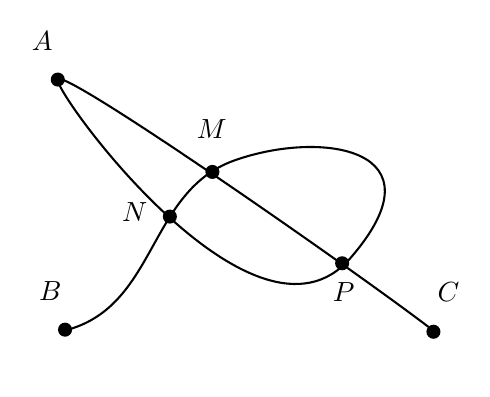
\begin{tikzpicture}[x=0.75pt,y=0.75pt,yscale=-1,xscale=1]
%uncomment if require: \path (0,300); %set diagram left start at 0, and has height of 300

%Curve Lines [id:da8281563189131769] 
\draw    (19,147.5) .. controls (64,136.5) and (59,80.5) .. (101,65.5) .. controls (143,50.5) and (203,59.5) .. (157,112.5) .. controls (111,165.5) and (14.5,33.25) .. (16,26.5) .. controls (17.5,19.75) and (162,120.5) .. (197,147.5) ;
%Shape: Circle [id:dp5537627399842162] 
\draw  [fill={rgb, 255:red, 0; green, 0; blue, 0 }  ,fill opacity=1 ] (13.13,26.5) .. controls (13.13,24.91) and (14.41,23.63) .. (16,23.63) .. controls (17.59,23.63) and (18.88,24.91) .. (18.88,26.5) .. controls (18.88,28.09) and (17.59,29.38) .. (16,29.38) .. controls (14.41,29.38) and (13.13,28.09) .. (13.13,26.5) -- cycle ;
%Shape: Circle [id:dp6514246924941245] 
\draw  [fill={rgb, 255:red, 0; green, 0; blue, 0 }  ,fill opacity=1 ] (16.63,147) .. controls (16.63,145.41) and (17.91,144.13) .. (19.5,144.13) .. controls (21.09,144.13) and (22.38,145.41) .. (22.38,147) .. controls (22.38,148.59) and (21.09,149.88) .. (19.5,149.88) .. controls (17.91,149.88) and (16.63,148.59) .. (16.63,147) -- cycle ;
%Shape: Circle [id:dp8776709133450113] 
\draw  [fill={rgb, 255:red, 0; green, 0; blue, 0 }  ,fill opacity=1 ] (194.13,148) .. controls (194.13,146.41) and (195.41,145.13) .. (197,145.13) .. controls (198.59,145.13) and (199.88,146.41) .. (199.88,148) .. controls (199.88,149.59) and (198.59,150.88) .. (197,150.88) .. controls (195.41,150.88) and (194.13,149.59) .. (194.13,148) -- cycle ;
%Shape: Circle [id:dp053192870659790614] 
\draw  [fill={rgb, 255:red, 0; green, 0; blue, 0 }  ,fill opacity=1 ] (150.13,115) .. controls (150.13,113.41) and (151.41,112.13) .. (153,112.13) .. controls (154.59,112.13) and (155.88,113.41) .. (155.88,115) .. controls (155.88,116.59) and (154.59,117.88) .. (153,117.88) .. controls (151.41,117.88) and (150.13,116.59) .. (150.13,115) -- cycle ;
%Shape: Circle [id:dp8447499185414264] 
\draw  [fill={rgb, 255:red, 0; green, 0; blue, 0 }  ,fill opacity=1 ] (87.63,71) .. controls (87.63,69.41) and (88.91,68.13) .. (90.5,68.13) .. controls (92.09,68.13) and (93.38,69.41) .. (93.38,71) .. controls (93.38,72.59) and (92.09,73.88) .. (90.5,73.88) .. controls (88.91,73.88) and (87.63,72.59) .. (87.63,71) -- cycle ;
%Shape: Circle [id:dp40686781525586535] 
\draw  [fill={rgb, 255:red, 0; green, 0; blue, 0 }  ,fill opacity=1 ] (67.13,92.5) .. controls (67.13,90.91) and (68.41,89.63) .. (70,89.63) .. controls (71.59,89.63) and (72.88,90.91) .. (72.88,92.5) .. controls (72.88,94.09) and (71.59,95.38) .. (70,95.38) .. controls (68.41,95.38) and (67.13,94.09) .. (67.13,92.5) -- cycle ;

% Text Node
\draw (2,2) node [anchor=north west][inner sep=0.75pt]   [align=left] {$\displaystyle A$};
% Text Node
\draw (5.5,122.5) node [anchor=north west][inner sep=0.75pt]   [align=left] {$\displaystyle B$};
% Text Node
\draw (197.5,123) node [anchor=north west][inner sep=0.75pt]   [align=left] {$\displaystyle C$};
% Text Node
\draw (147,123) node [anchor=north west][inner sep=0.75pt]   [align=left] {$\displaystyle P$};
% Text Node
\draw (81.5,44.5) node [anchor=north west][inner sep=0.75pt]   [align=left] {$\displaystyle M$};
% Text Node
\draw (45.5,84.5) node [anchor=north west][inner sep=0.75pt]   [align=left] {$\displaystyle N$};

\end{tikzpicture}
\end{center}

\noindent Sabendo-se que:
\begin{itemize}
    \item 17 carros passam por $M$, $N$ e $P$;
    \item 25 carros passam por $M$ e $P$;
    \item 28 carros passam por $N$ e $P$,
\end{itemize}
qual é o número total de carros?
\end{exer}
\begin{resp}
    36
\end{resp}

\begin{exer}
    Entre as pessoas que compareceram à uma festa de inauguração, estavam alguns dos amigos de Eduardo. Além disso, sabe-se que nem todos os melhores amigos de Eduardo foram à festa de inauguração. Considere:
\begin{itemize}
    \item F: conjunto de pessoas que foram à festa de inauguração.
    \item E: conjunto dos amigos de Eduardo.
    \item M: conjunto dos melhores amigos de Eduardo.
\end{itemize}
Com base nessas informações, represente o diagrama de Euler-Venn que descreve corretamente a relação entre os conjuntos.
\end{exer}

\begin{exer}
    Um conjunto $A$ tem 16 subconjuntos. Determine o número de elementos de $A$.
\end{exer}
\begin{resp}
    4
\end{resp}

\begin{exer}
    Sejam $A$, $B$, $C$ conjuntos finitos. O número de elementos de $A\cap B$ é 45; o número de elementos de $A\cap C$ é 40 e o número de elementos de $A\cap B\cap C$ é 25. Determine o número de elementos de $A\cap (B\cup C)$.
\end{exer}

\begin{exer}
    Se $A$ e $B$ são dois conjuntos não vazios, tais que $A-B=\{1,3,6,7\}$, $B-A=\{4,8\}$ e $A\cup B= \{1,2,3,4,5,6,7,8\}$, determine o conjunto $A\cap B$.
\end{exer}

\begin{exer}
    Dados os conjuntos $A=\{2,3\}$ e $B=\{3,4,5\}$, determine o conjunto $C$ tal que $A\cap C = \{2\}$, $B\cap C=\{4\}$ e $A\cup B\cup C=\{2,3,4,5,6\}$.
\end{exer}

\begin{exer}
    Classifique em verdadeiras (V) ou falsas (F) as sentenças a seguir:
    \begin{enumerate}[a)]
        \item $\{1\}\in\{1\}$
        \item $\{1\}\subset\{1\}$
        \item $1\in\{1\}$
        \item $\{1\}\in\{\{1\},\{2\}\}$
        \item $\{1\}\subset\{\{1\},\{2\}\}$
        \item $\varnothing\subset \varnothing$
        \item $\{1\}\subset\{1,\{1\}\}$
        \item $\varnothing\in\{1,\{1\},\{2\}\}$
        \item $\varnothing\subset\{1,\{1\},\{2\}\}$
        \item $\{\{1\}\}\subset\{1,\{1\},\{2\}\}$
        \item $\varnothing\in\{\varnothing, 1,\{1\}\}$
        \item $\varnothing\subset\{\varnothing, 1,\{1\}\}$
    \end{enumerate}
\end{exer}
% \begin{resp}
%     \par\noindent\rule{\columnwidth}{0.4pt}
% \end{resp}

%\subsection*{Respostas:}
%\noindent{\footnotesize \textit{*Em elaboração}}

%\shipoutAnswer

\end{secExercicios}